\chapter{实验结果与讨论}\label{ch:experiment}
本章从系统层面得分和句子层面得分两个方面展示了实验的数据与结论。
在众多数据中,我们发现以下主要的结论:
\begin{enumerate}
    \item 同一个数据集上的模型的得分差异较小,不同数据集上的模型得分差异较大。
    \item 各个指标的分布情况呈现集群现象,同一集群内的指标分布相似,不同集群之间的指标分布迥异。
    \item 尽管在某些指标或数据集上一个模型超过另一个模型,但是在全部指标和数据集上,没有哪个模型一致的超过另一个模型。
\end{enumerate}
我们把上述结论归因于以下几个方面:
\begin{enumerate}
    \item 合理的响应的空间巨大,响应具有很高的熵,给评价增加了难度。
    \item 模型在不同数据集上的泛化能力有待加强。
    \item 对话数据集的质量参差不齐,而模型的质量和数据集的质量紧密相关。
    \item 指标捕捉了错误的表征,不能正确反映模型的性能。
\end{enumerate}

% ------------------------- %
% ----- System Level ------ %
% ------------------------- %
\section{系统层面得分}\label{sec:system_scores}
表~\ref{tab:systemScoresAll}~展示了各个模型在不同数据集上测定的各项指标的系统层面得分,
加粗的得分是三个系统中的最优者。
句子平均长度(\#words)没有加粗,因为它是一个参考数据。
从表中的数据来看,
在LSDSCC上HRED取得了除ROUGE-4外所有指标的最优,
在OpenSubtitles上,VHRED取得了除了ADEM和Distinct-N之外所有指标
的最优,
在Ubuntu上情况比较复杂:HRED取得9个指标的最优,
LSTM取得了6个指标的最优,
VHRED取得了3个指标的最优。
如果我们把在一个数据集上取得最优指标最多的模型称为在该数据集上的
最优模型的话,
从总体上看,HRED是所有数据集上的最优模型,
因为它在LSDSCC和OpenSubtitles都是最优模型。
但是观察在每一项指标上取得最优的模型时我们发现,
不同数据集上的取得最优的模型往往不相同。
为了了解不同模型在不同数据集上的表现,
我们对每一个指标的系统层面得分绘制了柱形图。
\begin{table}%
\centering%
\caption{不同数据集上的模型的各种指标得分}%
\label{tab:systemScoresAll}%
\begin{tabular}{|l|l|l|l|l|l|l|l|l|l|}%
\hline%
&\multicolumn{3}{c|}{LSDSCC}&\multicolumn{3}{c|}{OpenSubtitles}&\multicolumn{3}{c|}{Ubuntu}\\%
\hline%
&HRED&LSTM&VHRED&HRED&LSTM&VHRED&HRED&LSTM&VHRED\\%
\hline%
ADEM&2.6178&2.6127&2.6163&2.6228&2.6224&2.6219&2.6353&2.6381&2.635\\%
\hline%
BLEU{-}1&0.08&0.0726&0.0722&0.0672&0.0638&0.0753&0.1314&0.1303&0.1365\\%
\hline%
BLEU{-}2&0.0264&0.0181&0.0185&0.0171&0.0153&0.0264&0.0362&0.0345&0.0375\\%
\hline%
BLEU{-}3&0.0105&0.0052&0.0066&0.0062&0.0055&0.0146&0.009&0.007&0.0089\\%
\hline%
BLEU{-}4&0.0053&0.0&0.0028&0.0024&0.0022&0.01&0.0029&0.0018&0.0025\\%
\hline%
Distinct{-}1&0.9577&0.9441&0.9558&0.973&0.9714&0.9714&0.9074&0.9257&0.9113\\%
\hline%
Distinct{-}2&0.8541&0.8511&0.8497&0.8669&0.8594&0.8665&0.9013&0.8603&0.8968\\%
\hline%
Greedy&0.3303&0.3292&0.3267&0.3102&0.2998&0.3145&0.2775&0.2364&0.273\\%
\hline%
Average&0.5532&0.5467&0.5483&0.5453&0.5295&0.5485&0.574&0.5205&0.5655\\%
\hline%
Extrema&0.2841&0.2835&0.2814&0.3009&0.2929&0.3061&0.29&0.2663&0.2875\\%
\hline%
METEOR&0.0296&0.0258&0.0281&0.0248&0.0233&0.0271&0.1657&0.1635&0.166\\%
\hline%
ROUGE{-}1&0.108&0.083&0.0978&0.0784&0.075&0.0872&0.1644&0.1836&0.1683\\%
\hline%
ROUGE{-}2&0.0226&0.0049&0.0081&0.0053&0.0043&0.0107&0.0128&0.0143&0.0128\\%
\hline%
ROUGE{-}3&0.0057&0.0002&0.0035&0.0011&0.0009&0.0053&0.0007&0.0003&0.0005\\%
\hline%
ROUGE{-}4&0.0011&0.0&0.003&0.0002&0.0002&0.0038&0.0002&0.0&0.0001\\%
\hline%
ROUGE{-}L&0.0956&0.0681&0.0846&0.0742&0.0707&0.0826&0.1493&0.1722&0.1535\\%
\hline%
ROUGE{-}W&0.0792&0.0537&0.07&0.066&0.0629&0.0734&0.1205&0.1391&0.1236\\%
\hline%
PPL&32.5599&32.9229&37.7149&41.6392&34.2724&33.6867&39.178&46.4061&40.2641\\%
\hline%
\#words&13.1605&14.0067&12.3612&8.807&8.6394&8.7798&23.0646&16.4905&21.2449\\%
\hline%
\end{tabular}%
\end{table}

% -- BLEU -- %
图~\ref{fig:BLEU_system}~是BLEU的系统得分柱形图。
BLEU-1和BLEU-2的情况比较类似:
从总体上看,模型在Ubuntu的得分普遍高于在另外两个数据集上的得分,
而HRED和VHRED在所有数据集上都比LSTM表现好,
在Ubuntu上,VHRED超过了HRED,但在另外两个数据集上,
HRED都一致的超过了VHRED。
模型的BLEU-1得分在虽然在不同数据集之间相差较大,
但在同一个数据集内却相差不大。
然而,模型的BLEU-2,BLEU-3,BLEU-4得分即便在同一个数据集内也相差很大。

BLEU-3和BLEU-4的情况比较类似:
从总体上看,没有哪一个数据集的得分要普遍高于其他数据集上的得分。
在所有数据集上,HRED和VHRED的得分仍然普遍比LSTM高,
虽然有时候优势不太明显 。
VHRED在OpenSubtitles上大幅度的超过了HRED,
但在另外两个数据集上,HRED都超过了VHRED。
从绝对数量的角度来看,BLEU的得分随着N的增大而减小,
这可能是因为两个句子的n-gram共现数随着$N$的增大而减少。
\begin{figure}[H]
    \begin{subfigure}{0.5\linewidth}
        \centering
        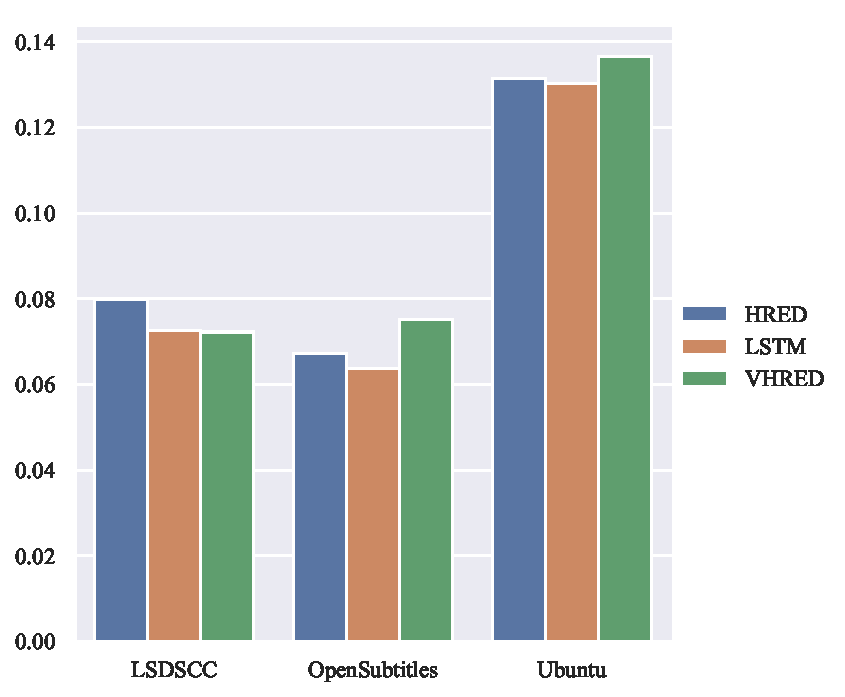
\includegraphics[width=\linewidth]{figure/barplot/bleu_1/plot.pdf}
        \caption{BLEU-1}
    \end{subfigure}%
    \begin{subfigure}{0.5\linewidth}
        \centering
        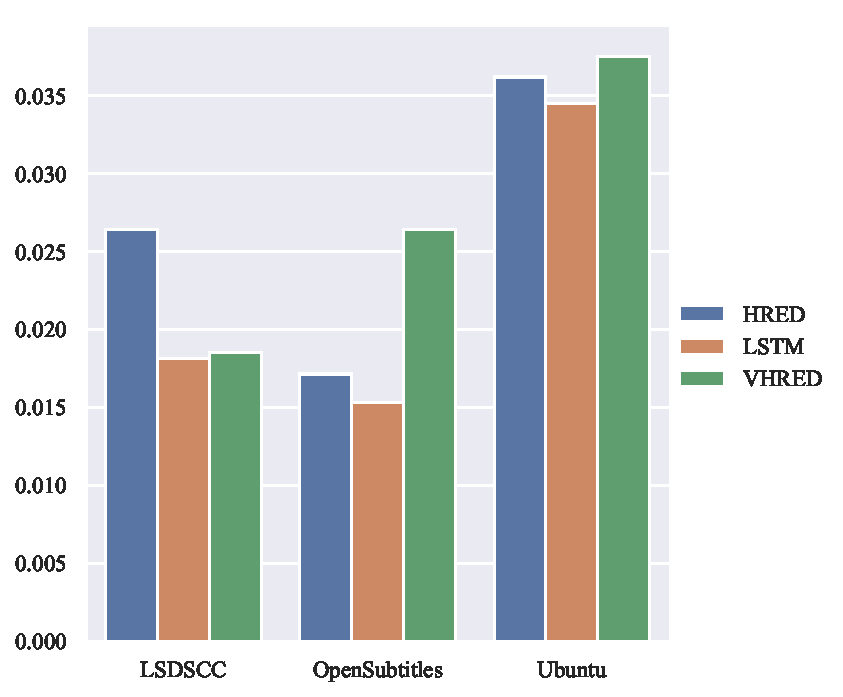
\includegraphics[width=\linewidth]{figure/barplot/bleu_2/plot.pdf}
        \caption{BLEU-2}
    \end{subfigure}
    \begin{subfigure}{0.5\linewidth}
        \centering
        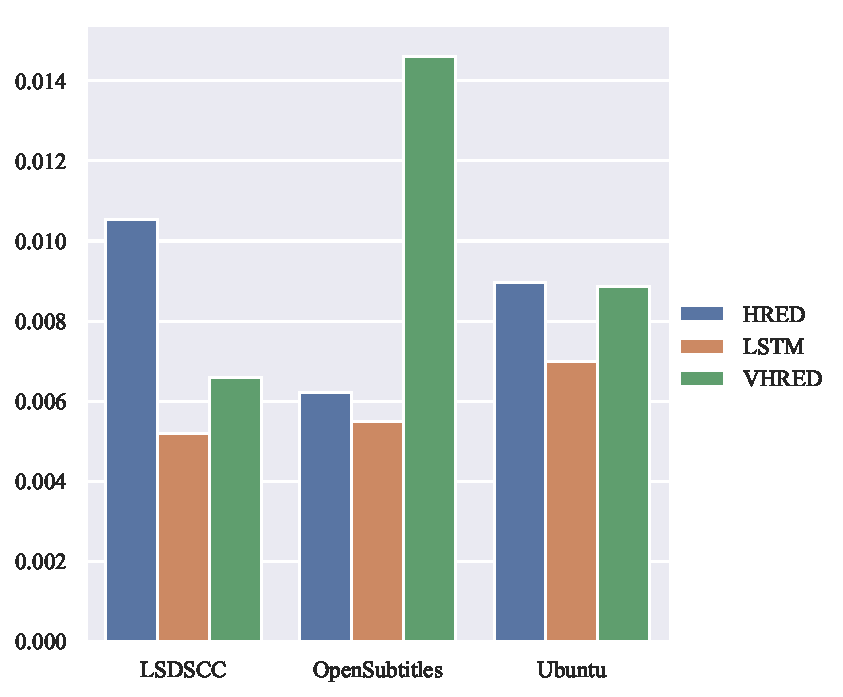
\includegraphics[width=\linewidth]{figure/barplot/bleu_3/plot.pdf}
        \caption{BLEU-3}
    \end{subfigure}%
    \begin{subfigure}{0.5\linewidth}
        \centering
        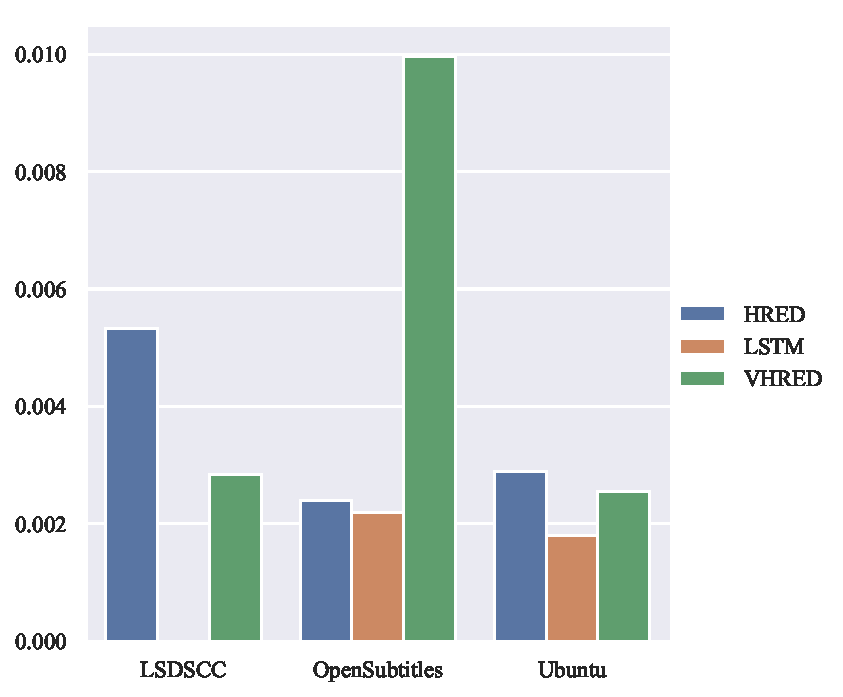
\includegraphics[width=\linewidth]{figure/barplot/bleu_4/plot.pdf}
        \caption{BLEU-4}
    \end{subfigure}
    \centering
    \caption{BLEU的系统得分}
    \label{fig:BLEU_system}
\end{figure}


% -- ADEM_AND_EMB -- %
图~\ref{fig:ADEM_EB_system}~是基于词嵌入的指标和ADEM的系统得分柱形图。
有趣的是,ADEM对所有数据集上的所有模型的打分都非常接近2.6。
从表~\ref{tab:ADEM_system}~看出,
当数据集不同时,ADEM的分数在百分位变化,
当数据集相同而模型不同时,ADEM的分数在千分位或之后变化,
这表明数据集对ADEM得分的影响要大于模型的影响。
\begin{table}
    \centering
    \caption{ADEM的系统层面打分}
    \label{tab:ADEM_system}
    \begin{tabular}{llll}
        \toprule
        & HRED & LSTM & VHRED \\
        \midrule
        LSDSCC & 2.6178 & 2.6127 & 2.6163  \\
        OpenSubtitles & 2.6228 & 2.6224 & 2.6219 \\
        Ubuntu & 2.6353 & 2.6381 & 2.635 \\
        \bottomrule
    \end{tabular}
\end{table}
从数据集的角度,所有模型在Ubuntu上的得分好于在OpenSubtitles的得分,
而后者要好于在LSDSCC上的得分。
从模型的角度,在LSDSCC上,HRED的得分好于VHRED的得分,
后者要好于LSTM的得分。
在OpenSubtitles上,HRED的得分好于LSTM的得分,
后者要好于VHRED的得分。
在Ubuntu上,最好的模型是LSTM,其次是HRED,最后是VHRED。
从上述分析来看,HRED在两个数据集上得分最优,
VHRED在两个数据集上得分最差,
LSTM在三个数据集上排名各不相同。
尽管得分的差异很小(最大值和最小值之间只相差0.019),
而且各个数据集上模型的排名都不相同,但是还是可以看出,
HRED在ADEM指标上表现较好,而VHRED则较差。
这可能是因为我们没有用预训练的HRED初始化VHRED。
\begin{figure}[H]
    \begin{subfigure}{0.45\linewidth}
        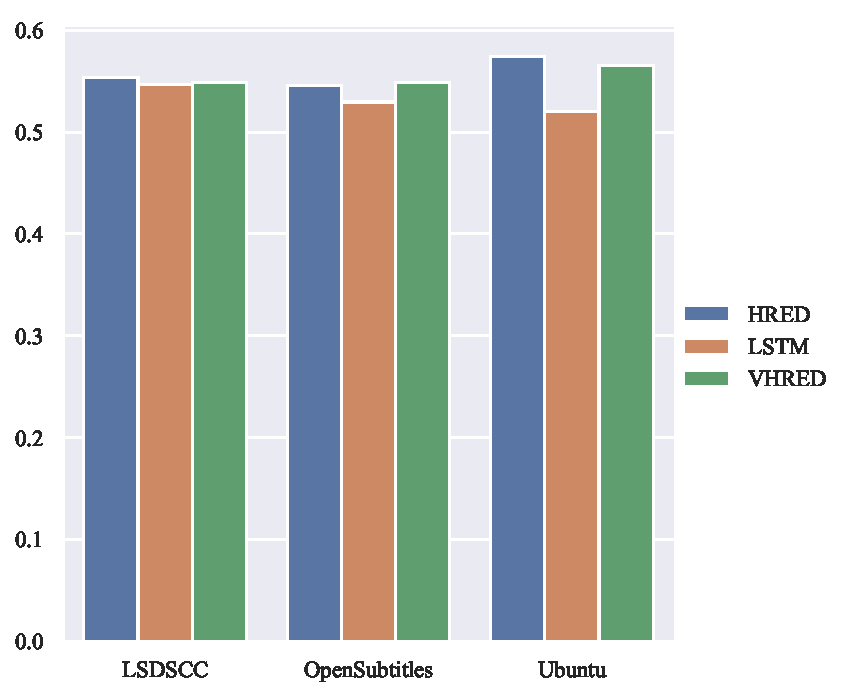
\includegraphics[width=\linewidth]{figure/barplot/embedding_based_vector_average/plot.pdf}
        \centering
        \caption{Average}
    \end{subfigure}%
    \begin{subfigure}{0.45\linewidth}
        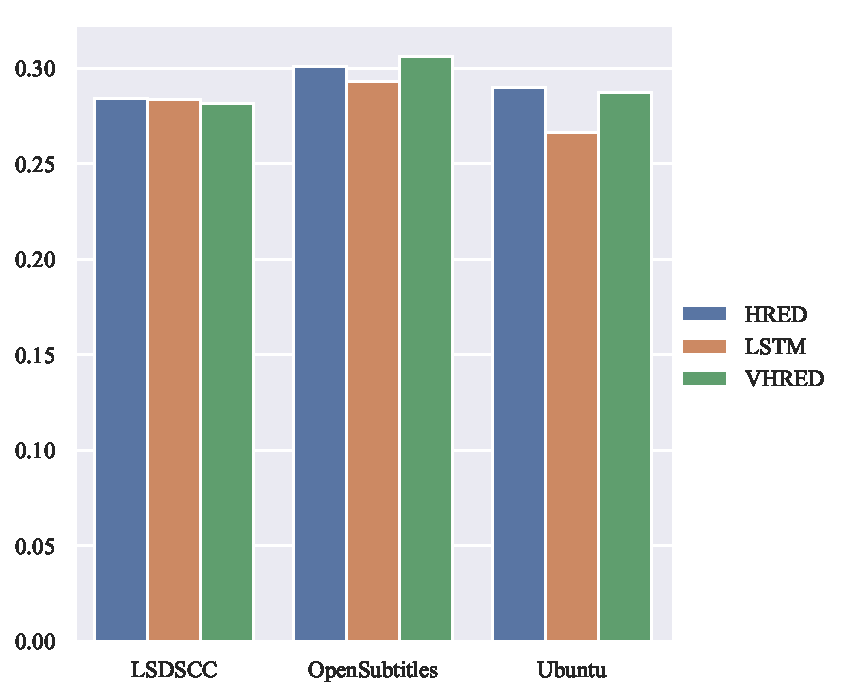
\includegraphics[width=\linewidth]{figure/barplot/embedding_based_vector_extrema/plot.pdf}
        \centering
        \caption{Extrema}
    \end{subfigure}
    \begin{subfigure}{0.45\linewidth}
        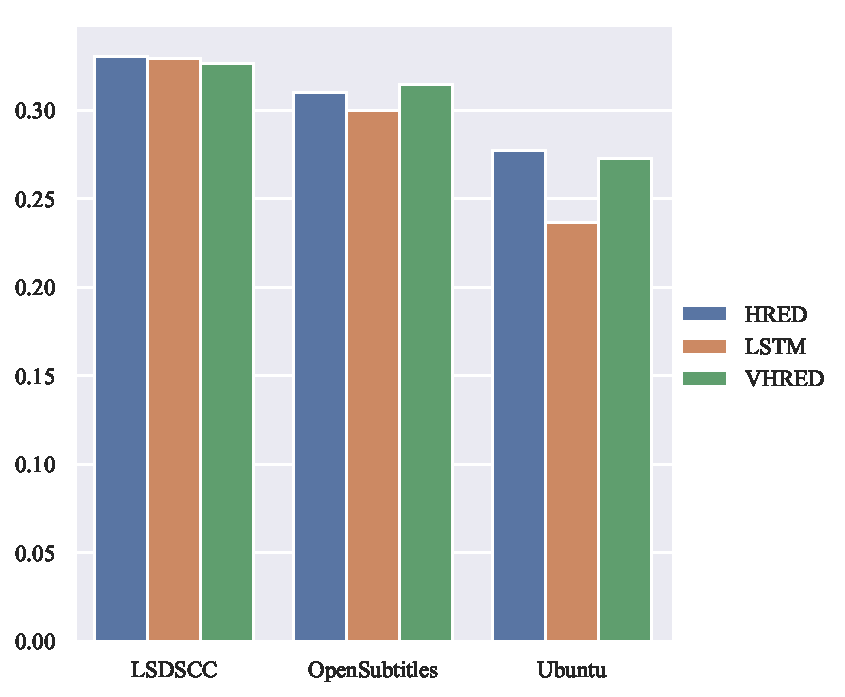
\includegraphics[width=\linewidth]{figure/barplot/embedding_based_greedy_matching/plot.pdf}
        \centering
        \caption{Greedy}
    \end{subfigure}%
    \begin{subfigure}{0.45\linewidth}
        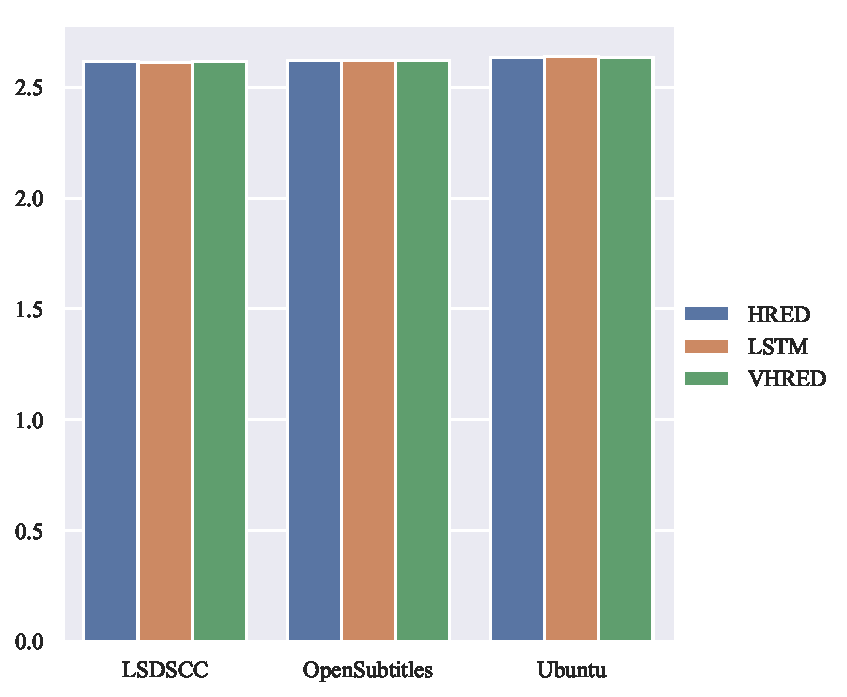
\includegraphics[width=\linewidth]{figure/barplot/adem/plot.pdf}
        \centering
        \caption{ADEM}
        \label{subfig:ADEM_system}
    \end{subfigure}
    \centering
    \caption{基于词嵌入的指标和ADEM的系统得分}
    \label{fig:ADEM_EB_system}
\end{figure}


和ADEM相比,基于词嵌入的指标表现的更具有一致性。
Average,Greedy和Extrema三种指标虽然在绝对数值上有些差异,
但是图像的模式却非常相似。
从总体来看,在所有数据集和指标上,HRED和VHRED都比LSTM表现的好。
我们发现在LSDSCC上,这三个指标很难将模型区分开来,
事实上,所有模型在LSDSCC上的某个指标都倾向于得到相同的分数。
我们猜测这是因为LSDSCC的测试集样本太少(300个),
没有足够多的样本令模型之间的差异展现出来。
在测试集样本数比较多的OpenSubtitles上,三个模型的区别比较明显,
但是由于OpenSubtitles的噪音比较大,话题比较分散,
模型相对比较容易产生话题相关的响应,
导致三个模型的区分不是特别明显。
在Ubuntu上,三个模型的区分最明显,
HRED和VHRED超过了LSTM,拉开了较大距离。
我们猜测这是因为Ubuntu是一个技术领域的数据集,
含有大量技术词汇,如\texttt{apt-get},\texttt{java}等等。
模型必须能捕捉到消息中的技术相关的语义并生成相关的句子才能的高分,
这要求模型对消息的主题有很强的捕捉能力。
HRED和VHRED比LSTM多了编码器结构,可以肯定它们捕捉消息主题的能力更强。
此外,模型在三个数据集上的区分度的不同也和数据集的对话轮数有关,
LSDSCC是单轮对话,OpenSubtitles是3轮对话,而Ubuntu是多轮对话。
多轮对话数据集更有利于能够利用它们的HRED和VHRED。

% -- ROUGE -- %
\begin{figure}[H]
    \begin{subfigure}{0.5\linewidth}
        \centering
        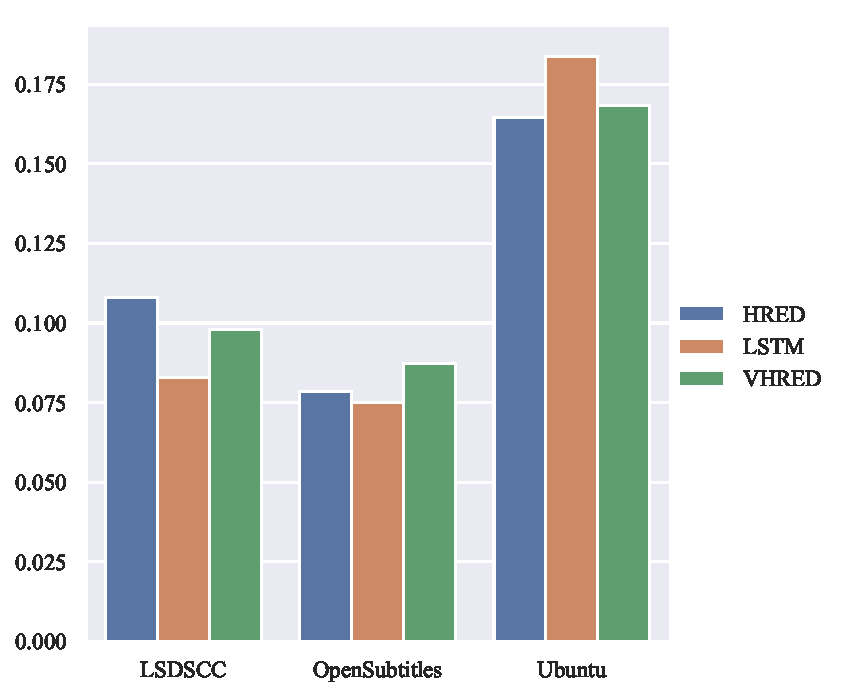
\includegraphics[width=\linewidth]{figure/barplot/rouge_1/plot.pdf}
        \caption{ROUGE-1}
    \end{subfigure}%
    \begin{subfigure}{0.5\linewidth}
        \centering
        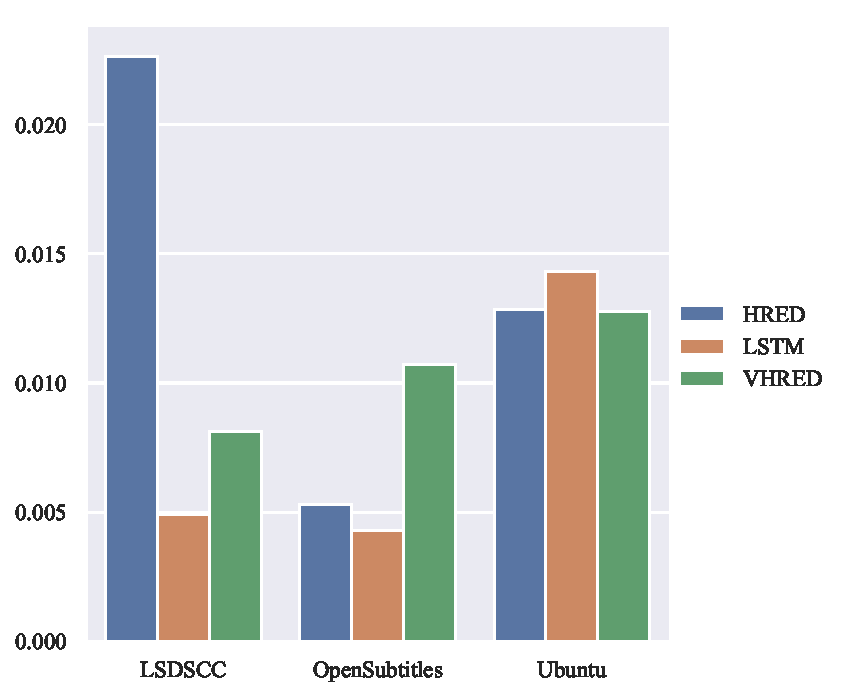
\includegraphics[width=\linewidth]{figure/barplot/rouge_2/plot.pdf}
        \caption{ROUGE-2}
    \end{subfigure}
    \begin{subfigure}{0.5\linewidth}
        \centering
        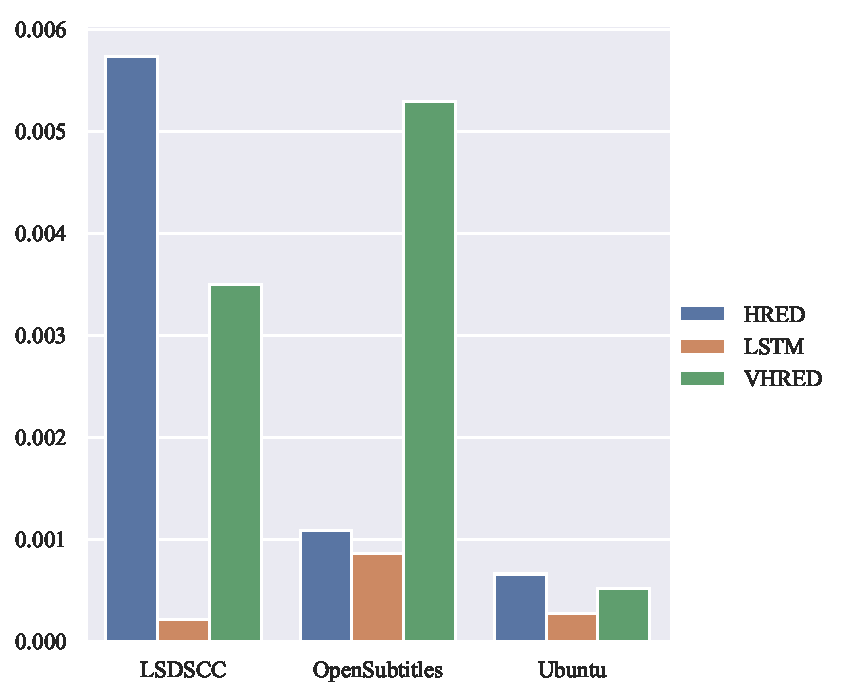
\includegraphics[width=\linewidth]{figure/barplot/rouge_3/plot.pdf}
        \caption{ROUGE-3}
    \end{subfigure}%
    \begin{subfigure}{0.5\linewidth}
        \centering
        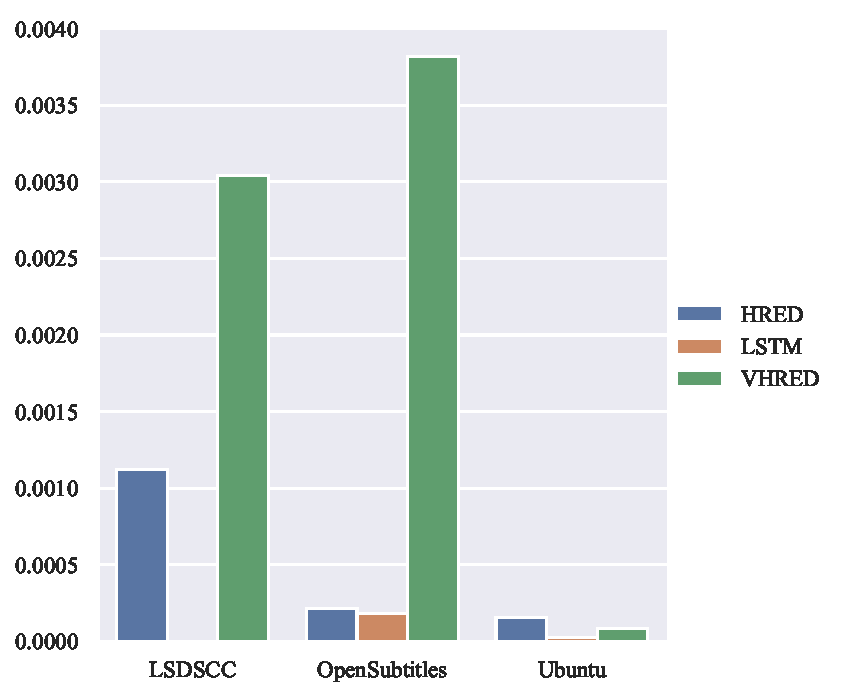
\includegraphics[width=\linewidth]{figure/barplot/rouge_4/plot.pdf}
        \caption{ROUGE-4}
    \end{subfigure}
    \centering
    \begin{subfigure}{0.5\linewidth}
        \centering
        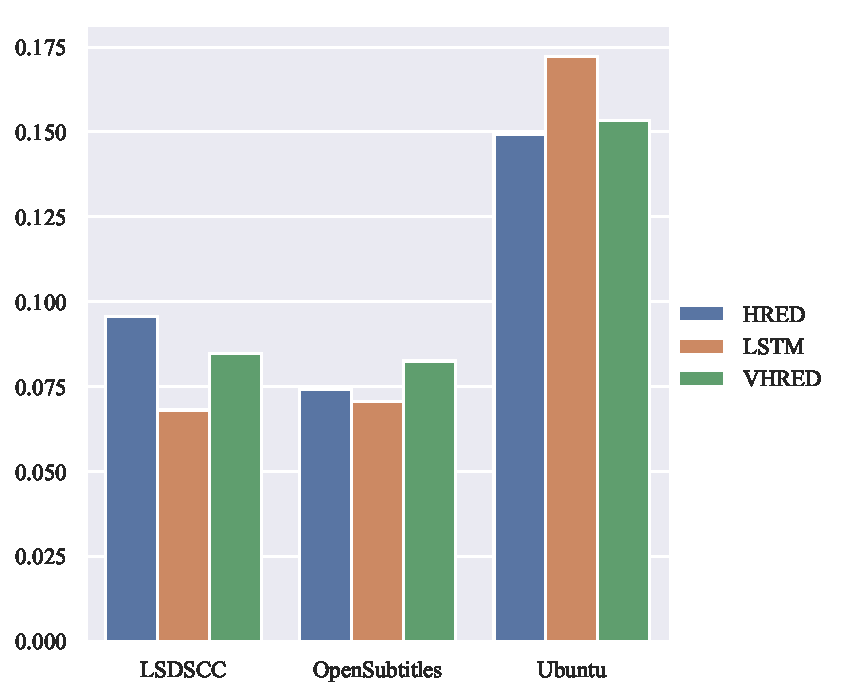
\includegraphics[width=\linewidth]{figure/barplot/rouge_l/plot.pdf}
        \caption{ROUGE-L}
    \end{subfigure}%
    \begin{subfigure}{0.5\linewidth}
        \centering
        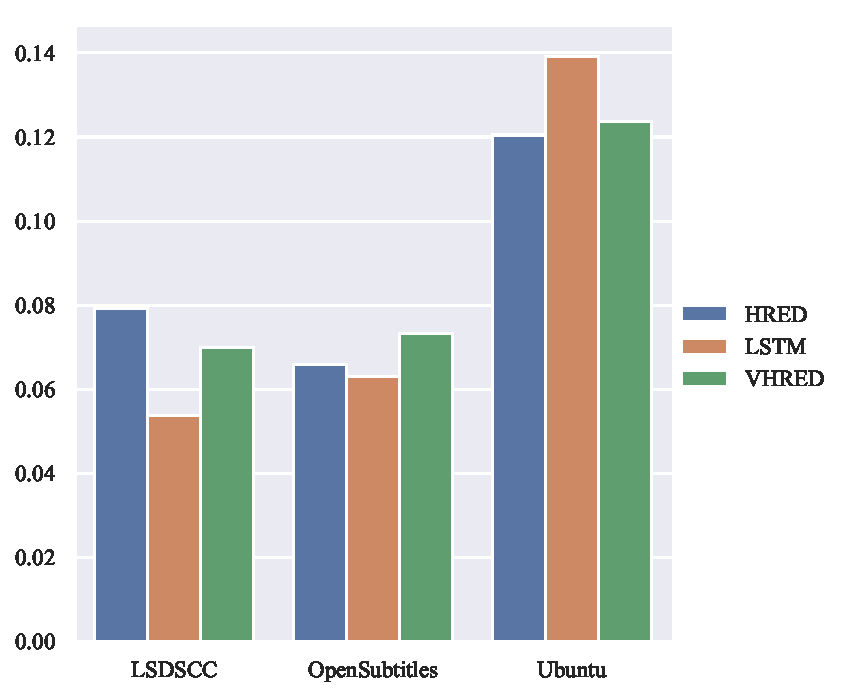
\includegraphics[width=\linewidth]{figure/barplot/rouge_w/plot.pdf}
        \caption{ROUGE-W}
    \end{subfigure}
    \centering
    \caption{ROUGE-L和ROUGE-W的系统得分}
    \label{fig:ROUGE_LW_system}
\end{figure}

图~\ref{fig:ROUGE_system}~是ROUGE的系统得分柱形图。
从总体上看,
不同数据集上的模型在ROUGE-1,ROUGE-2,ROUGE-L和ROUGE-W的得分都不为0,
但在ROUGE-3和ROUGE-4上,多个模型的得分接近0,
这是正常的,因为一般来说,响应和参考之间的高阶n-gram重叠非常少。
ROUGE-1,ROUGE-L和ROUGE-W的图像非常相似。
在这三个指标上,在LSDSCC和OpenSubtitles上,HRED和VHRED超过了LSTM,
但在Ubuntu上,LSTM却超过了HRED和VHRED;
除此之外,各个数据集内三个模型的排名也基本一致,
但是模型之间的差距有时很大,比如LSDSCC上的ROUGE-2,
有时很小,比如OpenSubtitles上的ROUGE-1。

在ROUGE-3和ROUGE-4上,LSTM的得分在所有数据集上普遍很低,
而HRED和VHRED在某些数据集上得分也很低,
在Ubuntu上,所有模型的得分都很低。
令人注目的是,VHRED在OpenSubtitles和LSDSCC上都取得了不错的成绩,
而HRED的表现在LSDSCC上较好,在OpenSubtitles上较差。

% -- Other -- %
图~\ref{fig:Other_system}~是Distinct-N,
METEOR和句子长度的系统得分图。
在Ubuntu上的模型的句子长度明显大于
在LSDSCC上的模型,而后者大于在OpenSubtitles上的模型。
从第~\ref{sec:dataset_proprecessing}~节我们知道,
训练集的平均句子长度有Ubuntu 大于 LSDSCC 大于 OpenSubtitles。
模型生成的响应的长度和训练集的平均句子长度具有一致性,
这是因为训练的目标函数是最大化训练集样本的对数概率,
所以模型倾向于模仿训练集的统计特征。

Distinct-N对模型的区分度不高,
在同一个数据集上训练的模型,它们的Distinct-N都比较接近。
从数据集的角度,OpenSubtitles上的模型的Distinct-1较高,
而Ubuntu上的模型的Distinct-2较高。
METEOR似乎受句子长度的影响较大,
在句子长度较大的Ubuntu上,模型的METEOR得分要比其他数据集上的得分高得多。
而LSDSCC上的METEOR也比OpenSubtitles上的得分略高。
METEOR对不同模型的区分度不是很大,
但从总体上看,HRED和VHRED比LSTM的表现要好。
\begin{figure}[H]
    \begin{subfigure}{0.5\linewidth}
        \centering
        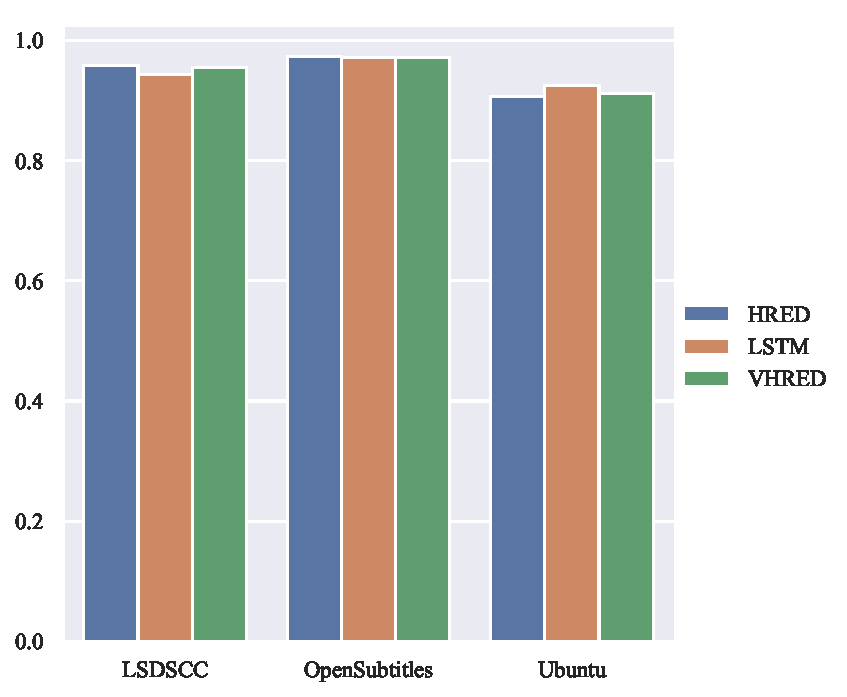
\includegraphics[width=\linewidth]{figure/barplot/distinct_1/plot.pdf}
        \caption{Distinct-1}
        \label{fig:distinct_1_system}
    \end{subfigure}%
    \begin{subfigure}{0.5\linewidth}
        \centering
        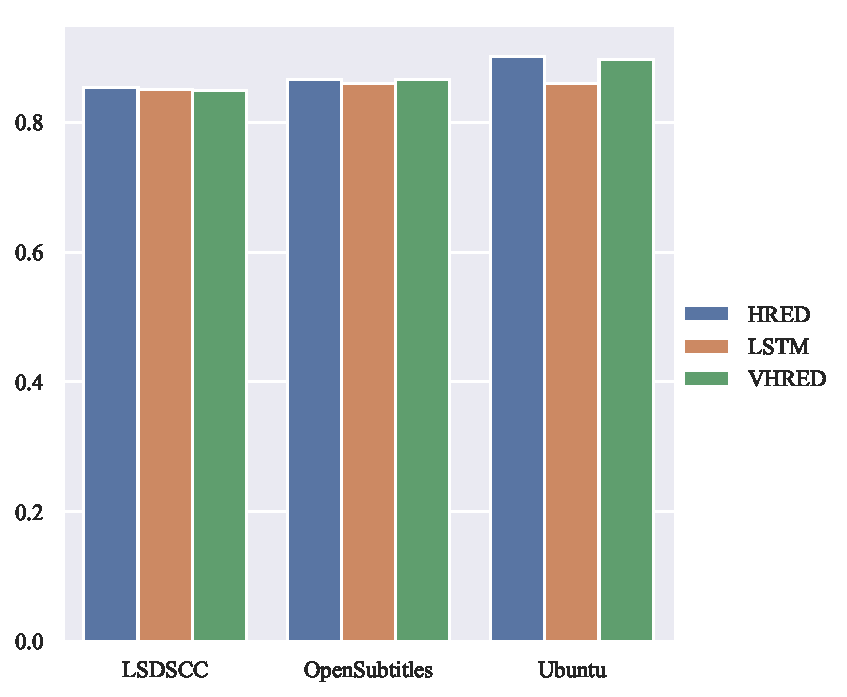
\includegraphics[width=\linewidth]{figure/barplot/distinct_2/plot.pdf}
        \caption{Distinct-2}
        \label{fig:distinct_2_system}
    \end{subfigure}

    \begin{subfigure}{0.5\linewidth}
        \centering
        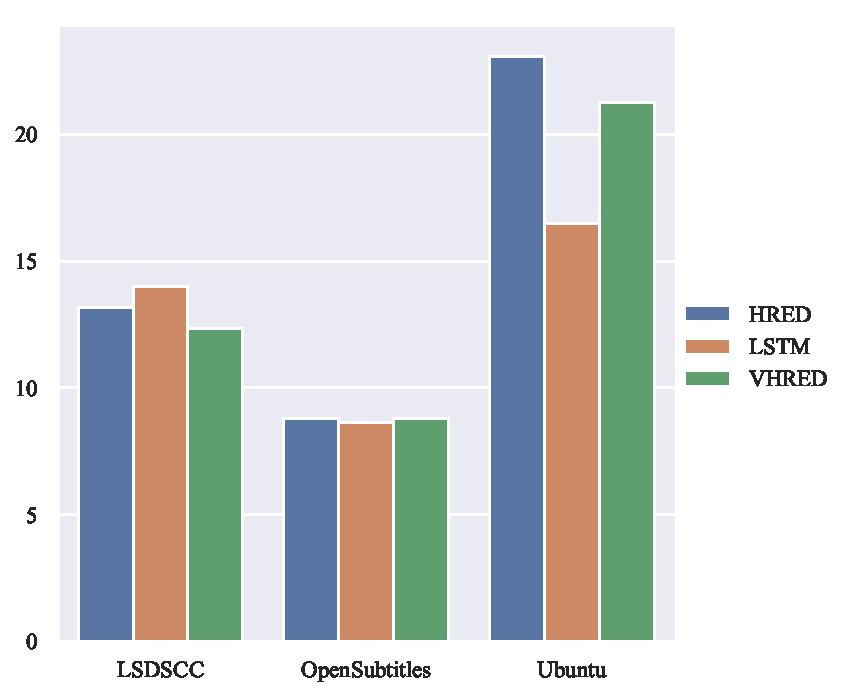
\includegraphics[width=\linewidth]{figure/barplot/utterance_len/plot.pdf}
        \caption{\#words}
        \label{fig:words_system}
    \end{subfigure}%
    \begin{subfigure}{0.5\linewidth}
        \centering
        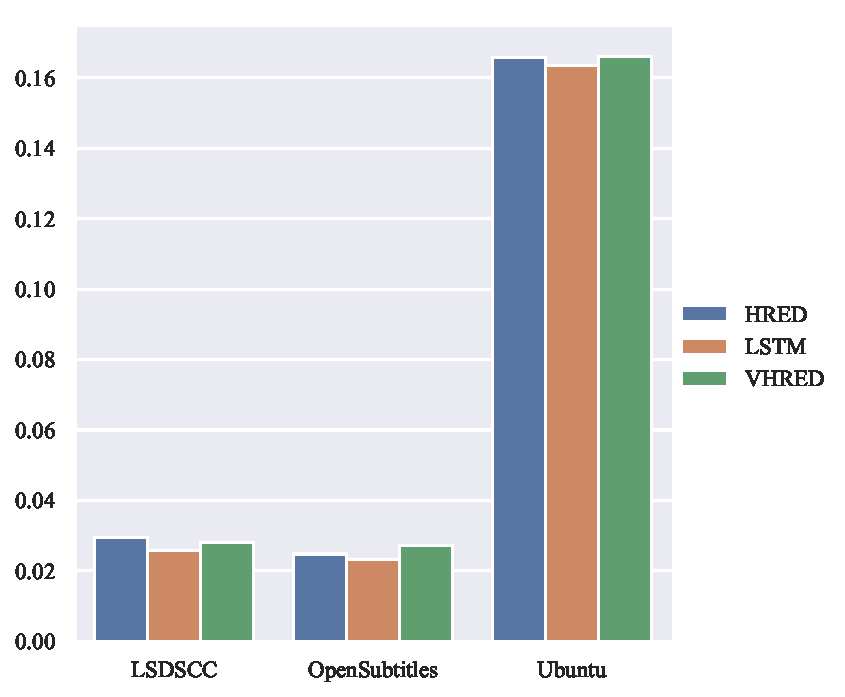
\includegraphics[width=\linewidth]{figure/barplot/meteor/plot.pdf}
        \caption{METEOR}
        \label{fig:meteor_system}
    \end{subfigure}
    \caption{Distinct-N,\#words和METEOR的系统得分}
    \label{fig:Other_system}
\end{figure}


% -- Conclusion -- %
本节利用柱状图分析了模型,数据集和指标的系统层面得分。
在一些图中,各个模型或者数据集的得分差异不十分明显,
为了突显得分的差异,我们把观察的维度分成数据集和模型两个维度,
并分别绘制了箱体图。
通过箱体图得出的结论是相同的,但是由于图像的数量较多,所以放在了附录。
附录~\ref{ch:dataset_system_dist}~从
数据集的维度 和 模型的维度 展示了不同指标的系统层面得分。

% --------------------- %
% -- Utterance Level -- %
% --------------------- %
\section{句子层面得分}\label{sec:utterance_scores}
我们还从句子层面得分方面进行了分析。
因为模型生成的句子$u$可以看做一个句子空间$U$上的随机变量,
而指标是一个确定的函数$f_{s}$,
所以可以把句子层面的得分看做一个随机变量$\lambda_u = f_{s}(u)$。
于是我们便可以用描述统计学(Descriptive Statistics)和统计推断断(Statistical Inference)
的方法来分析指标在句子水平的情况。

我们绘制了各种指标的句子层面得分的单变量分布(Univariate Distribution)。
为了便于从图像上比较各种指标的分布特征,我们对数值作了归一化处理,
使数据的平均值为0,标准差为1:
\begin{align}
    x' = \frac{x - \mu}{\sigma}
\end{align}
$\mu$是$x$的平均值,$\sigma$是$x$的标准差。
为了使读者能快速检阅所有指标的分布情况,
我们在正文展示了模型为HRED,数据集为OpenSubtitles的各项指标的分布,
附录~\ref{ch:metric_dist}~展示了所有的组合上的指标分布。

% -- BLEU -- %
\begin{figure}[H]
    \begin{subfigure}{0.5\linewidth}
        \centering
        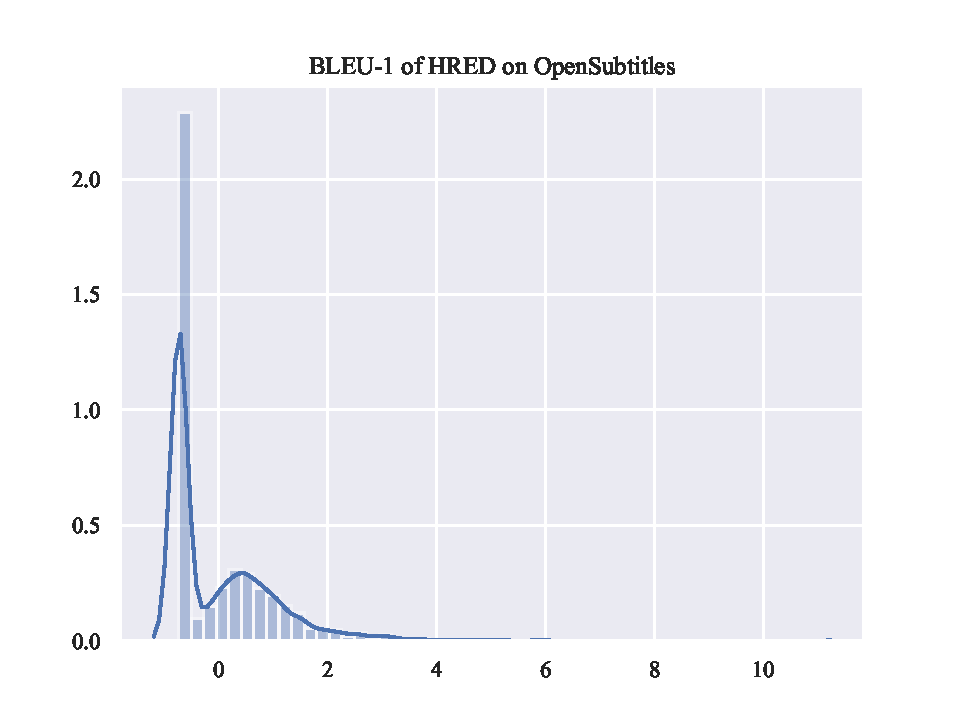
\includegraphics[width=\linewidth]{figure/distplot/opensub/hred/bleu_1/plot.pdf}
        \caption{BLEU-1}
    \end{subfigure}%
    \begin{subfigure}{0.5\linewidth}
        \centering
        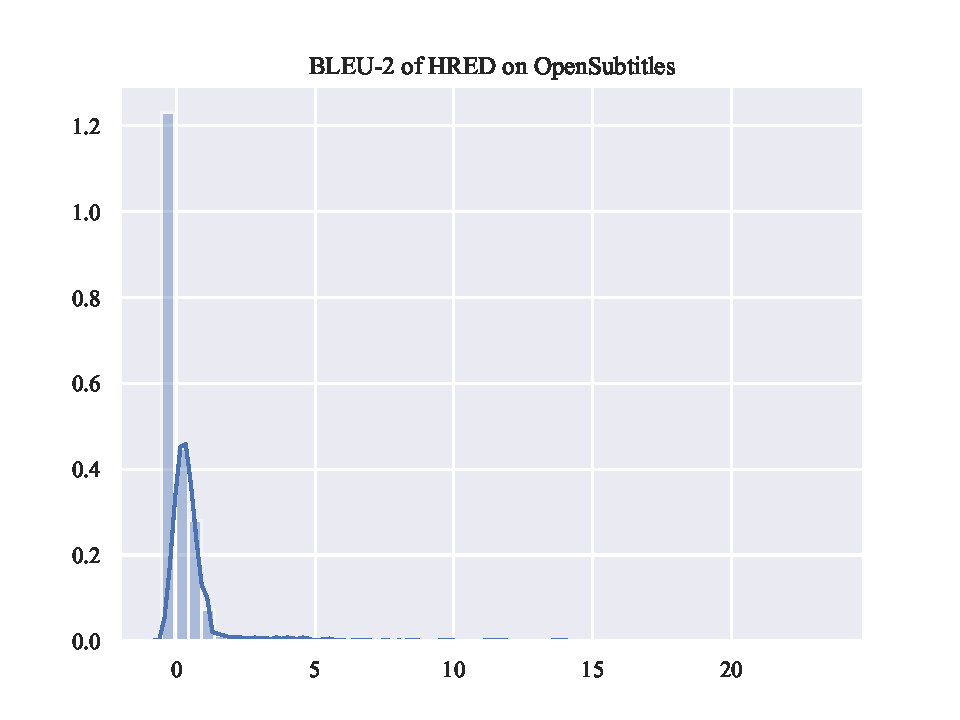
\includegraphics[width=\linewidth]{figure/distplot/opensub/hred/bleu_2/plot.pdf}
        \caption{BLEU-2}
    \end{subfigure}
    \begin{subfigure}{0.5\linewidth}
        \centering
        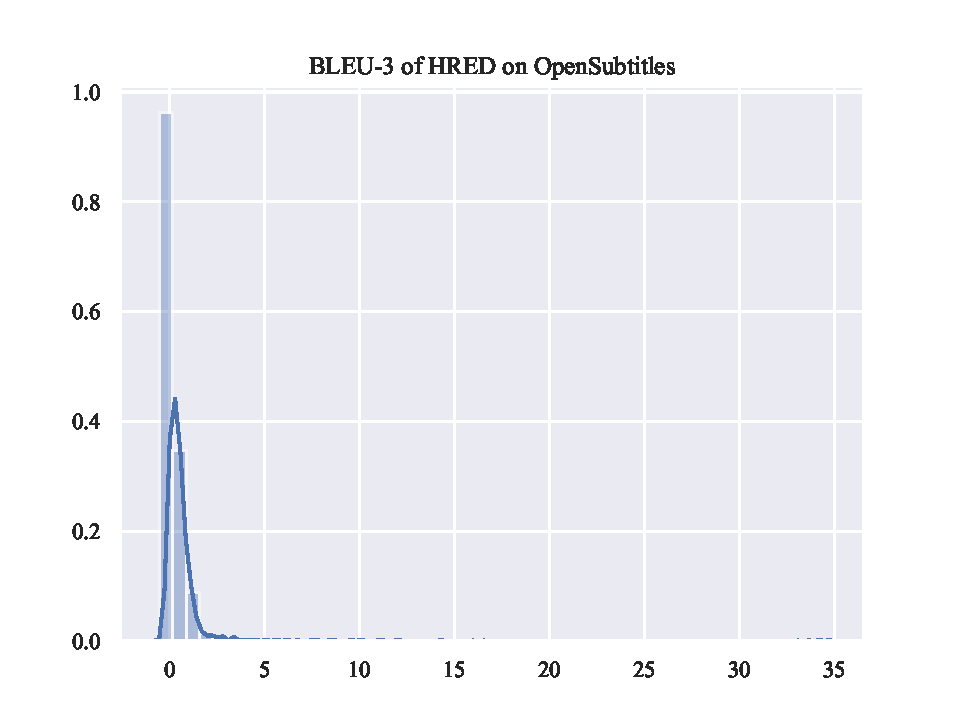
\includegraphics[width=\linewidth]{figure/distplot/opensub/hred/bleu_3/plot.pdf}
        \caption{BLEU-3}
    \end{subfigure}%
    \begin{subfigure}{0.5\linewidth}
        \centering
        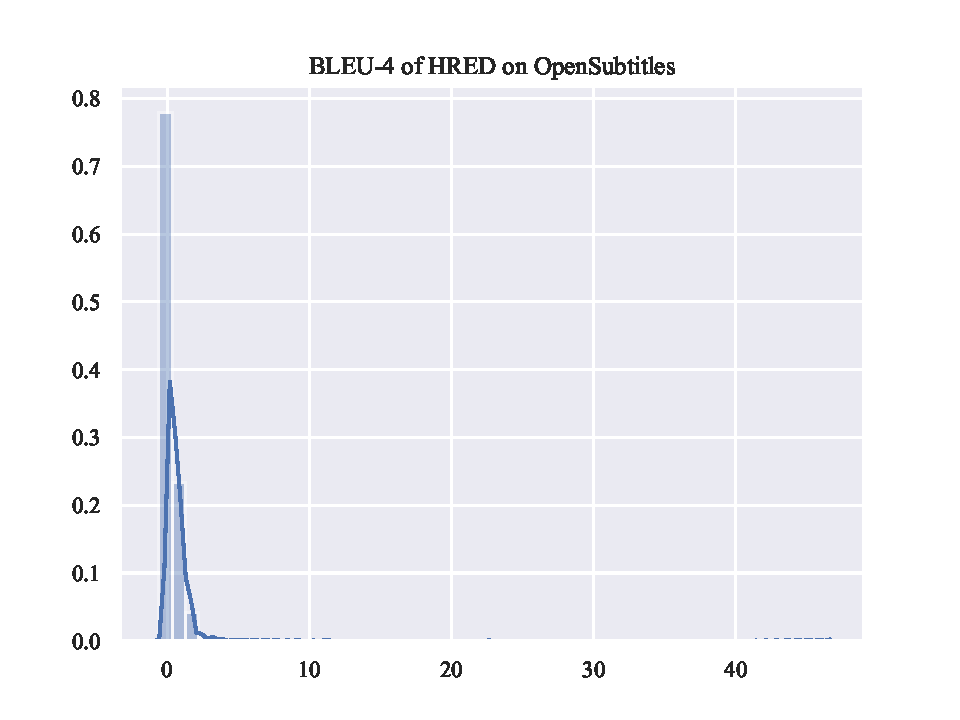
\includegraphics[width=\linewidth]{figure/distplot/opensub/hred/bleu_4/plot.pdf}
        \caption{BLEU-4}
    \end{subfigure}
    \centering
    \caption{BLEU的概率分布图}
    \label{fig:BLEU_dist}
\end{figure}

图~\ref{fig:BLEU_dist}~是BLEU的N取1到4时的分布图。
由于加入了平滑处理,所以大部分得分都有非零数值,
在均值附近集中了大量的句子,
这可能是因为大部分句子的得分非常低\upcite{HowNot}。
一元词匹配相对高阶n-gram匹配更容易,
所以BLEU-1在均值的右边有一个低矮的峰值,
并且峰值对应的横坐标偏离了均值0,
这说明有相当一部分句子的得分高于均值。
而低于均值的部分出现了一个高峰,说明也有大量句子得分低于均值。
BLEU-2至4的分布都非常相似,
只是峰值的横坐标比BLEU-1更接近均值。
从总体上来说,BLEU的分布形状十分尖锐,大量句子集中在均值附近,
图像不对称, 峰值比高斯分布的峰值$1 / \sqrt{2 \pi} \approx 0.4$高。

% -- ADEM_AND_EMB -- %
\begin{figure}[H]
    \begin{subfigure}{0.5\linewidth}
        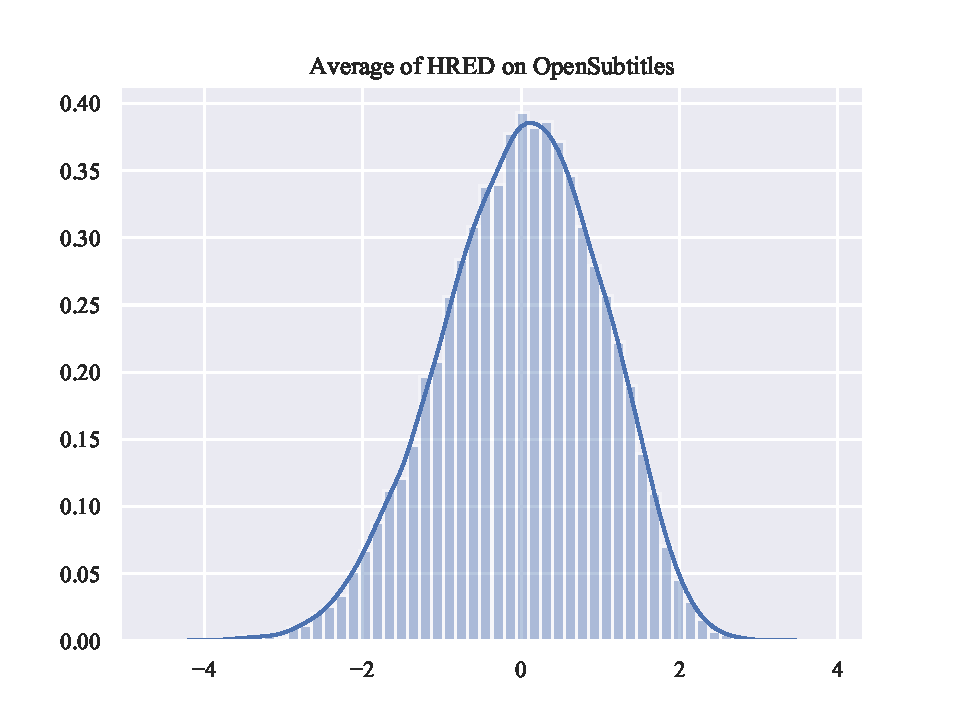
\includegraphics[width=\linewidth]{figure/distplot/opensub/hred/embedding_based_vector_average/plot.pdf}
        \centering
        \caption{Average}
    \end{subfigure}%
    \begin{subfigure}{0.5\linewidth}
        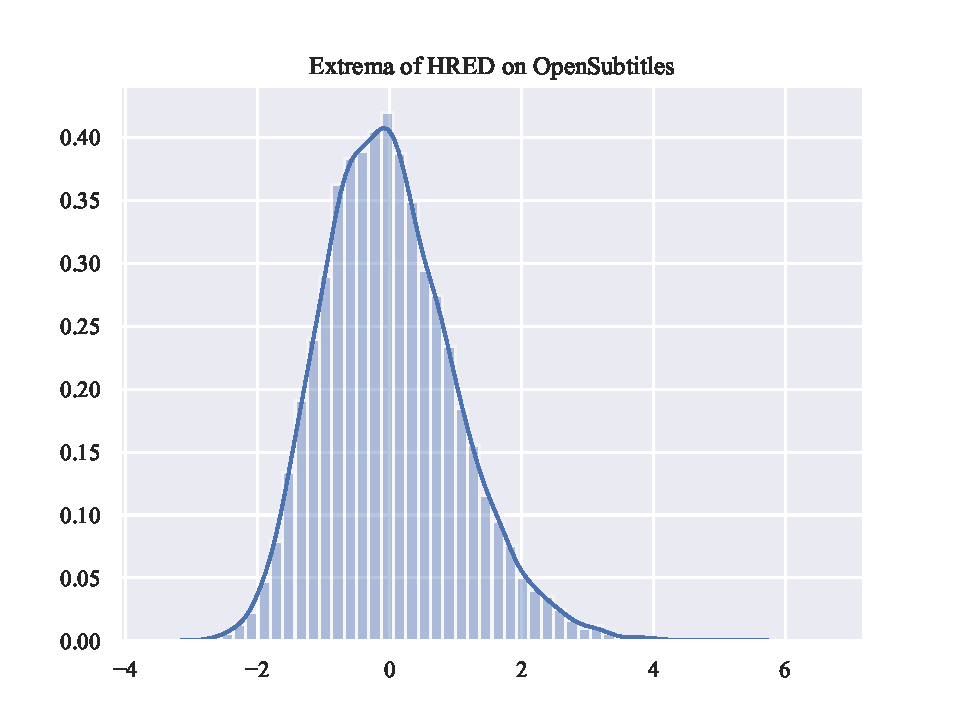
\includegraphics[width=\linewidth]{figure/distplot/opensub/hred/embedding_based_vector_extrema/plot.pdf}
        \centering
        \caption{Extrema}
    \end{subfigure}
    \begin{subfigure}{0.5\linewidth}
        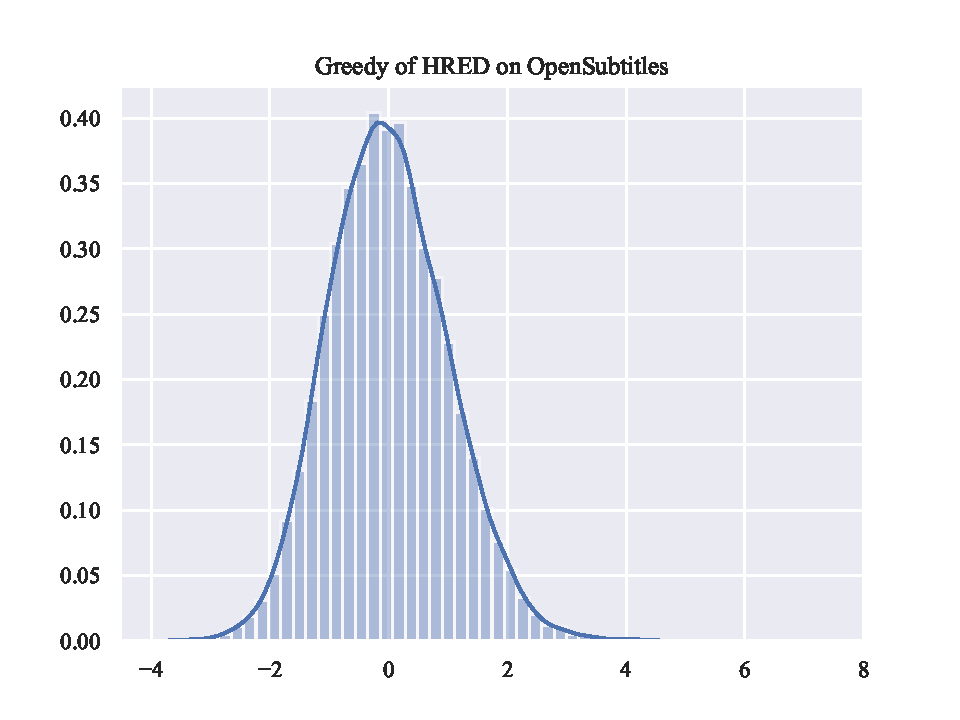
\includegraphics[width=\linewidth]{figure/distplot/opensub/hred/embedding_based_greedy_matching/plot.pdf}
        \centering
        \caption{Greedy}
    \end{subfigure}%
    \begin{subfigure}{0.5\linewidth}
        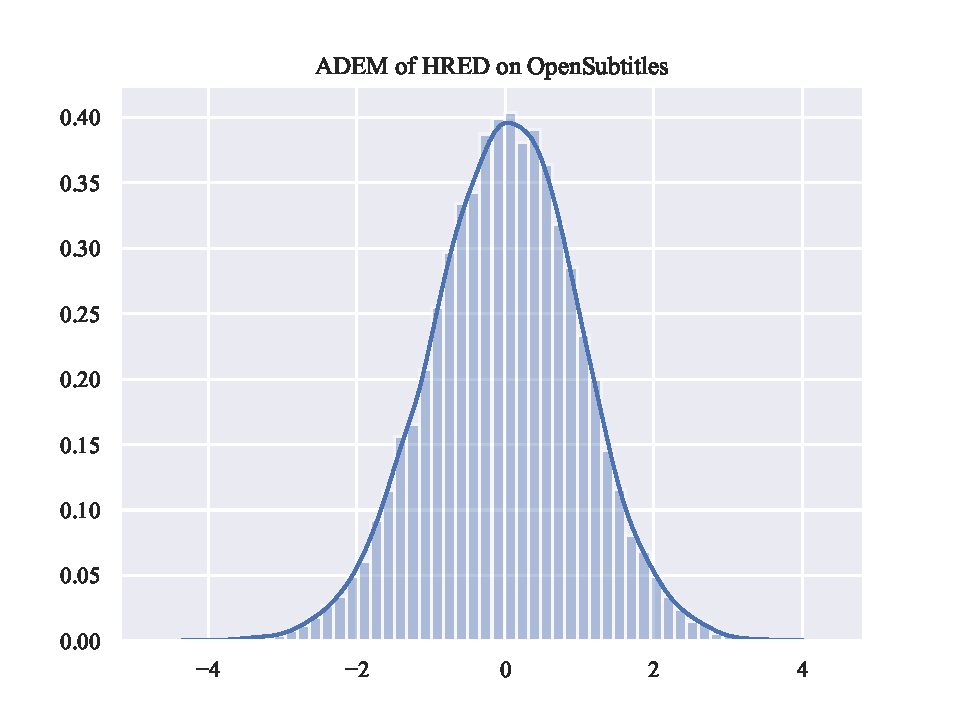
\includegraphics[width=\linewidth]{figure/distplot/opensub/hred/adem/plot.pdf}
        \centering
        \caption{ADEM}
    \end{subfigure}
    \caption{基于词嵌入的指标和ADEM的概率分布}
    \label{fig:ADEM_EB_dist}
\end{figure}

图~\ref{fig:ADEM_EB_dist}~是基于词嵌入的指标和ADEM指标的分布图。
因为ADEM可以看做是一种更高级的词嵌入指标,所以把它和其他词嵌入指标并列。
四个图像均呈钟型曲线,峰值非常接近0.4,峰值的横坐标则非常接近0。
ADEM曲线显示出几乎完美的对称,Greedy曲线的对称度次之,
Average曲线向右边偏移,Extrema曲线向左边偏移。
ADEM和词嵌入指标有相似之处。
从句子向量的组合方式来看,
Average的组合方法是平均值,Extrema的组合方法是极端值,
而ADEM的则使用了预训练的VHRED的编码器。
与其他词嵌入指标不同的是,ADEM考虑了上下文的影响,
用神经网络对上下文,响应和参考三者加权,
并且显式的优化了和人类评价的相关性,
可见ADEM采用的机制更为复杂。
Lowe在\upcite{ADEM}中指出,ADEM倾向于保守打分,
即人类评价给高分的句子,ADEM倾向于给稍低的分数。
从ADEM的曲线可以从某种意义上验证这一点,
得分高于平均值的句子与得分低于平均值的句子几乎一样多,
说明它不倾向于打高分或者低分。

% -- ROUGE -- %
\begin{figure}[H]
    \begin{subfigure}{0.5\linewidth}
        \centering
        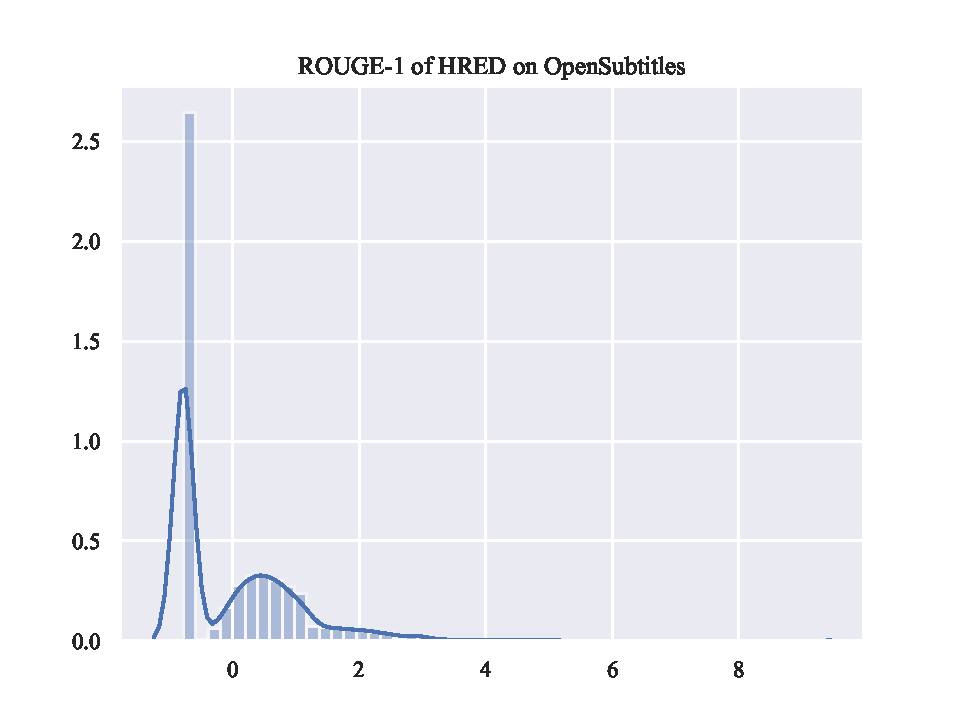
\includegraphics[width=\linewidth]{figure/distplot/opensub/hred/rouge_1/plot.pdf}
        \caption{ROUGE-1}
    \end{subfigure}%
    \begin{subfigure}{0.5\linewidth}
        \centering
        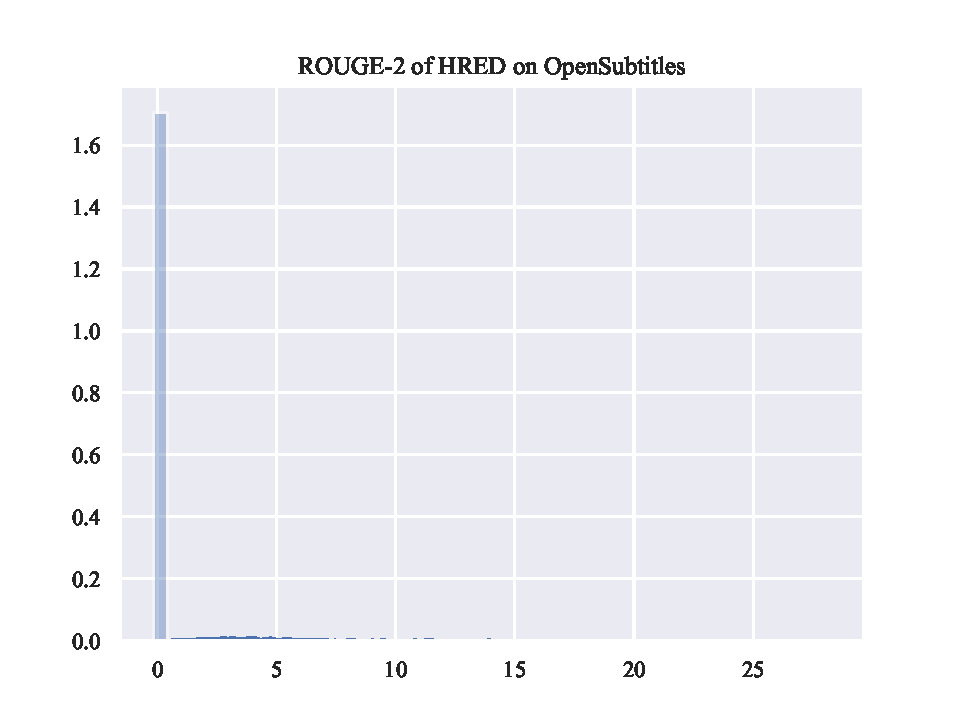
\includegraphics[width=\linewidth]{figure/distplot/opensub/hred/rouge_2/plot.pdf}
        \caption{ROUGE-2}
    \end{subfigure}
    \begin{subfigure}{0.5\linewidth}
        \centering
        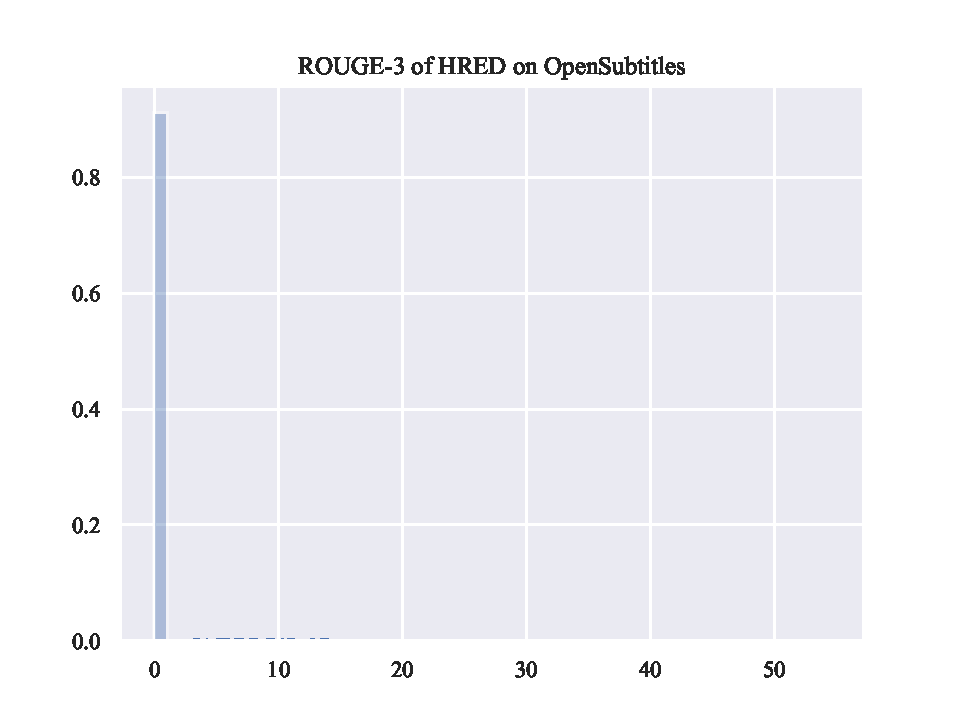
\includegraphics[width=\linewidth]{figure/distplot/opensub/hred/rouge_3/plot.pdf}
        \caption{ROUGE-3}
    \end{subfigure}%
    \begin{subfigure}{0.5\linewidth}
        \centering
        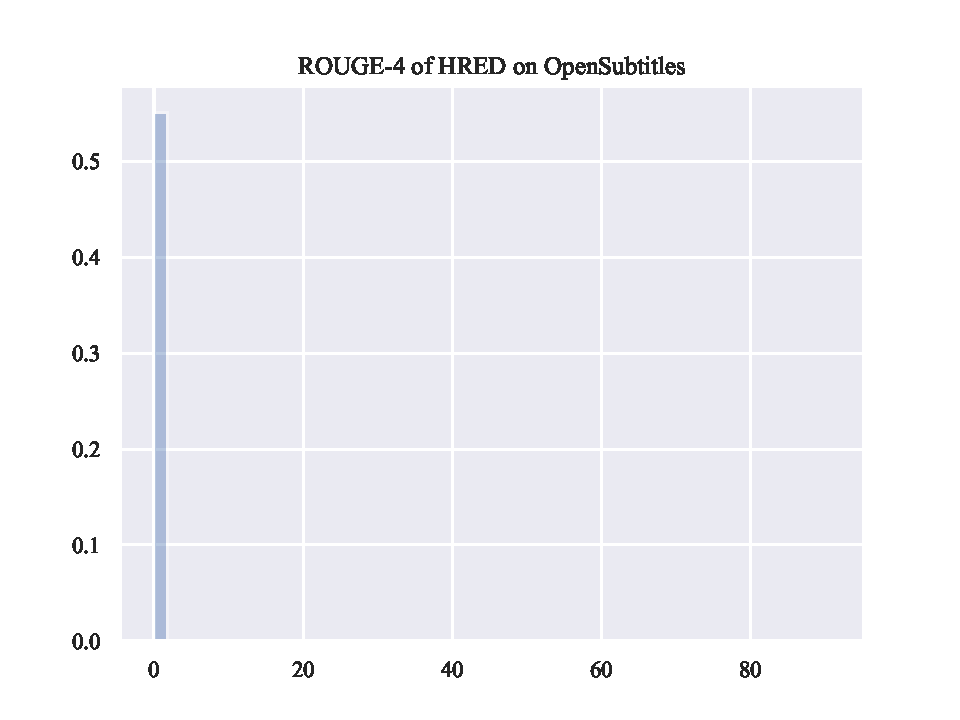
\includegraphics[width=\linewidth]{figure/distplot/opensub/hred/rouge_4/plot.pdf}
        \caption{ROUGE-4}
    \end{subfigure}
    \centering
    \begin{subfigure}{0.5\linewidth}
        \centering
        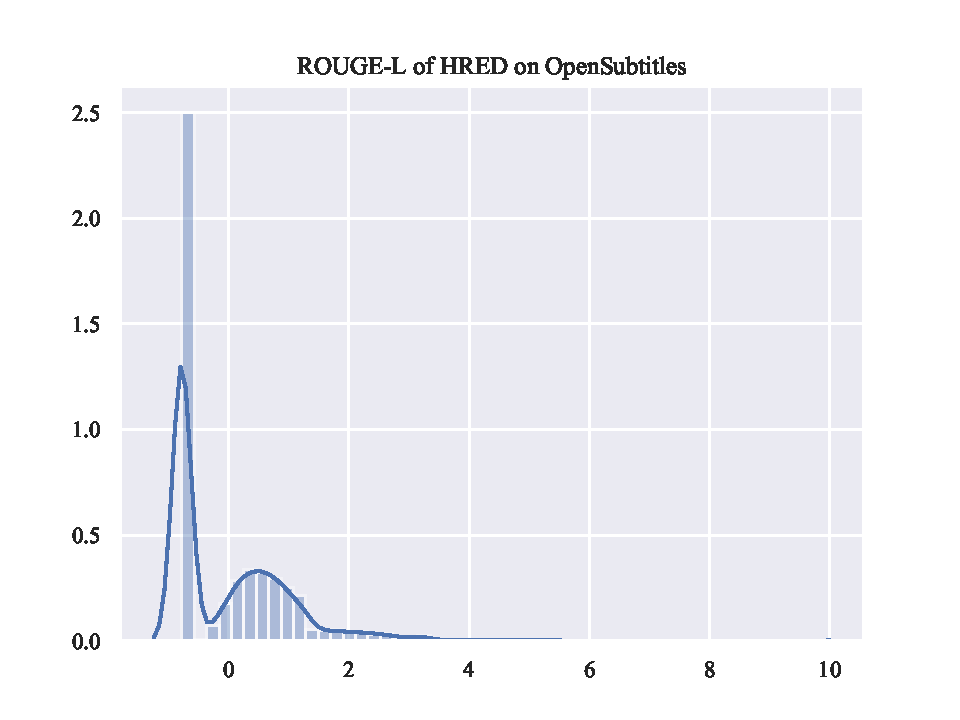
\includegraphics[width=\linewidth]{figure/distplot/opensub/hred/rouge_l/plot.pdf}
        \caption{ROUGE-L}
    \end{subfigure}%
    \begin{subfigure}{0.5\linewidth}
        \centering
        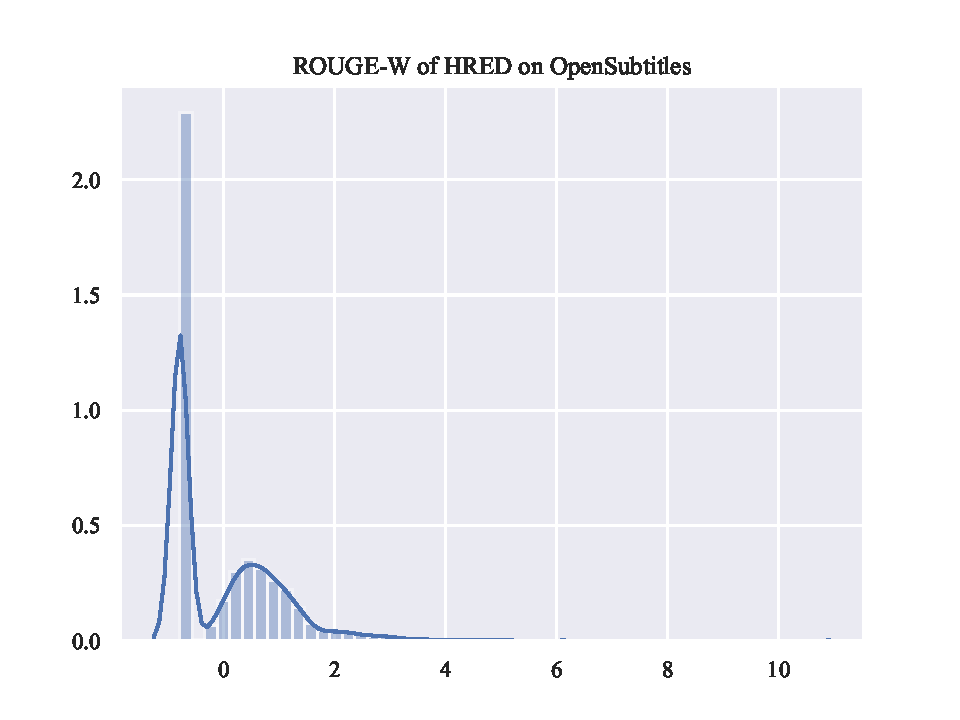
\includegraphics[width=\linewidth]{figure/distplot/opensub/hred/rouge_w/plot.pdf}
        \caption{ROUGE-W}
    \end{subfigure}
    \centering
    \caption{ROUGE的概率分布}
    \label{fig:ROUGE_dist}
\end{figure}

图~\ref{fig:ROUGE_dist}~是ROUGE系列指标的分布图。
从曲线的形状来看,大致可分为两类:
ROUGE-1,ROUGE-L,ROUGE-W是一类,
ROUGE-2,ROUGE-3,ROUGE-4是一类。
ROUGE-2这类图像的特点是几乎所有句子的得分都集中在均值,
除此之外没有其他得分。
我们猜想因为没有对ROUGE指标做任何平滑处理,除了极个别句子外,
其他句子都得了零分。
这表明ROUGE-N指标当$N > 1$时捕捉不到任何n-gram重叠。

另一方面,ROUGE-1类指标更像是BLEU-1指标的噪化版本,
它们都是双峰曲线,而且第一个峰值对应的点$(x_1, y_1)$和
第二个峰值对应的点$(x_2, y_2)$都有相似的坐标。
我们猜想上述现象的原因是所有的响应和参考基本上没有$N > 1$的n-gram重叠,
因此基于最长公共子序列的匹配退化成了一元词匹配。

% -- Other -- %
图~\ref{fig:Other_dist}~是Distinct-N,METEOR和\#words的分布图。
我们发现Distinct-1的分布呈现两极分化,
在均值附近和均值右边较远处都聚集了大量句子。
Distinct-N的分母是句子的长度(\#words),
分子是句子中各异的n-gram数量。
从\ref{fig:words_dist}来看,句子的长度集中在均值附近,
长于均值的句子比短于均值的句子多,
这表明Distinct-N的值主要受分子影响。
Distinct-1的曲线表明,极大部分句子的各异的单词数量都接近平均值,
但也有少部分句子各异的单词数量远远小于平均值。
% -- Distinct-2
Distinct-2的图像没有出现两极分化,
可能是因为二元词的空间比一元词的空间更大,
一个句子各异的二元词通常多余各异的一元词。
图像的特点是:
\begin{enumerate}
    \item 大部分句子集中在高于均值的一片区域。
    \item 个别低于均值的区间聚集了大量句子。
\end{enumerate}
这可以理解为模型在应对不同的消息时,
生成的句子质量不一,对一部分消息产生了多样的响应,
对另一部分消息却产生了单调的响应。
\begin{figure}[H]
    \begin{subfigure}{0.5\linewidth}
        \centering
        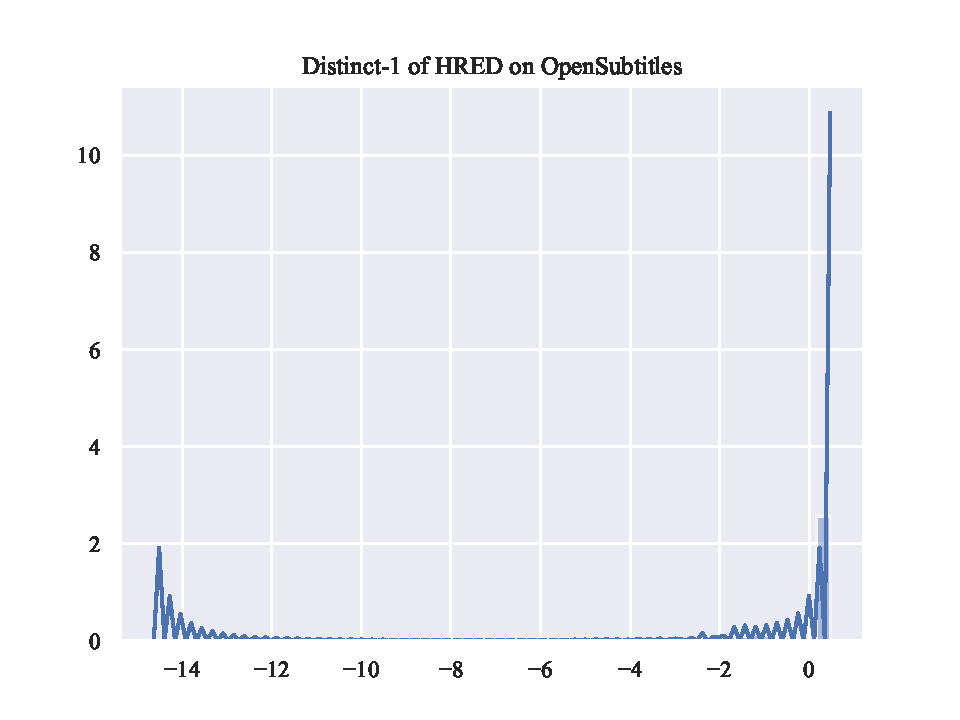
\includegraphics[width=\linewidth]{figure/distplot/opensub/hred/distinct_1/plot.pdf}
        \caption{Distinct-1}
    \end{subfigure}%
    \begin{subfigure}{0.5\linewidth}
        \centering
        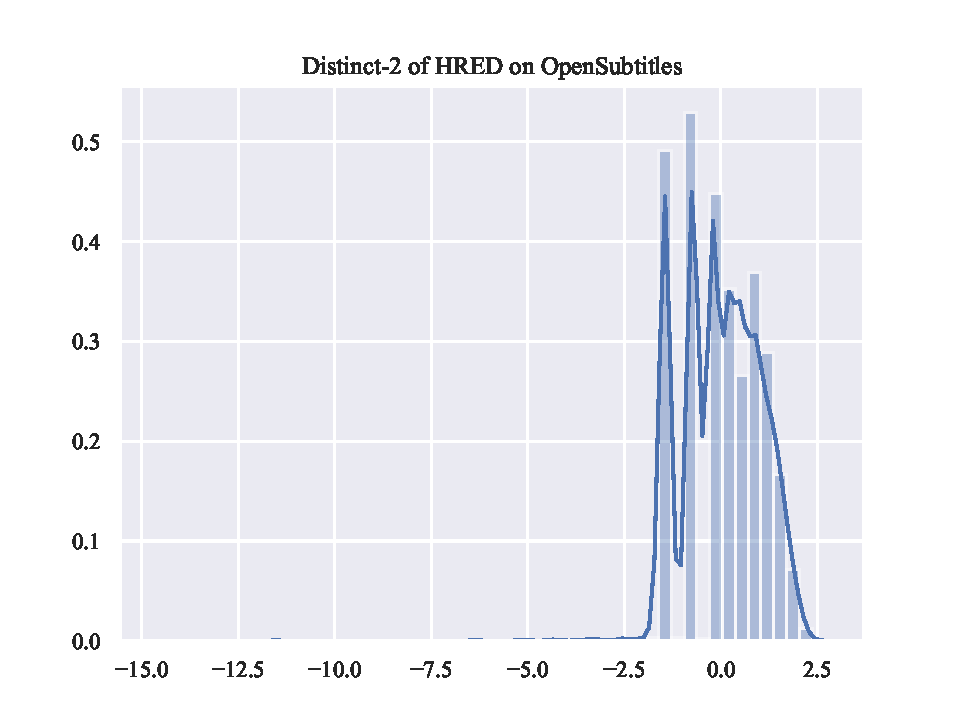
\includegraphics[width=\linewidth]{figure/distplot/opensub/hred/distinct_2/plot.pdf}
        \caption{Distinct-2}
    \end{subfigure}

    \begin{subfigure}{0.5\linewidth}
        \centering
        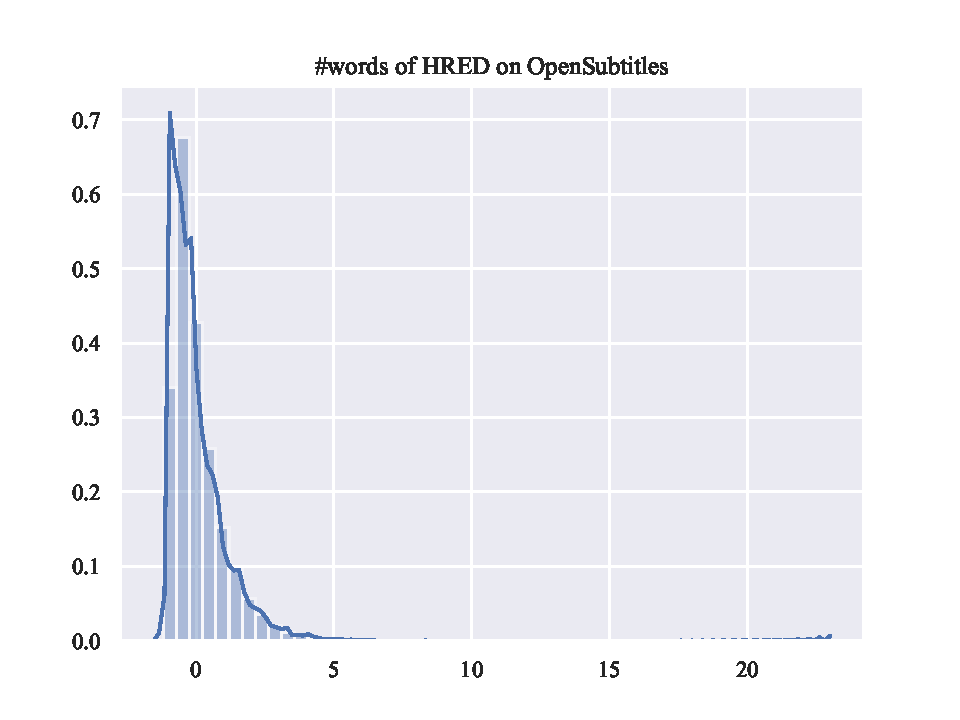
\includegraphics[width=\linewidth]{figure/distplot/opensub/hred/utterance_len/plot.pdf}
        \caption{#words}
    \end{subfigure}%
    \begin{subfigure}{0.5\linewidth}
        \centering
        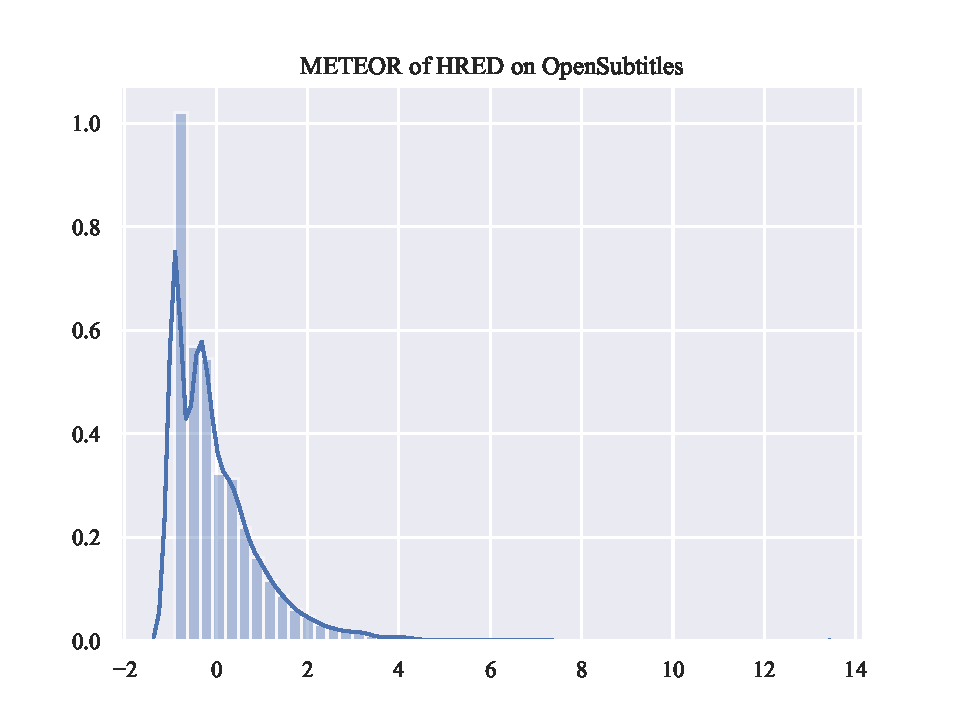
\includegraphics[width=\linewidth]{figure/distplot/opensub/hred/meteor/plot.pdf}
        \caption{METEOR}
    \end{subfigure}
    \caption{Distinct-N,#words和METEOR的概率分布图}
    \label{fig:Other_dist}
\end{figure}


% -- METEOR -- %
尽管通常被分类成基于词重叠的指标,
METEOR的图像表现出了和其他基于词重叠的指标(BLEU,ROUGE)相当不同的性质。
它似乎能区分不同响应的质量,并且和句子长度有着某种联系。
图像在均值的右侧表现出指数衰减, 在左侧则是一个尖锐的单峰。
本质上,METEOR是基于一元词匹配的,
但是我们尚不清楚METEOR的多种匹配模块,对齐算法和惩罚系数如何
使它的分布变得与BLEU-1等指标的分布如此不同。

% -- Conclusion -- %
中心极限定理(Central Limit Theorems)表明:
大量独立随机变量的叠加近似于高斯分布。
我们假设当句子足够多时,句子层面的人类评价近似于高斯分布。
据此我们认为,句子层面得分的分布接近高斯分布是一个指标
和人类评价具有较高相关性的前提条件之一。
从上述各个指标的分布来看, ADEM和词嵌入指标具有很大的潜力。

本节的分析结果是从OpenSubtitles和HRED的组合中得出的,
并不能完全代表所有组合下的指标分布情况。
观察附录~\ref{ch:metric_dist}可发现, 一般来说,
指标的分布当模型不同而数据集相同时比较相似,
当模型相同而数据集不同时则有较大差异,
因此句子层面的指标分布受数据集的影响较大。

% ---------------- %
% -- Discussion -- %
% ---------------- %
\section{结果与讨论}\label{sec:result_and_discussion}
% -- System Level -- %
通过系统层面的分析,我们发现数据集对指标的影响普遍大于模型的影响,
表现为同一个数据集上的模型得分比较接近,
同一个模型在不同数据集上的得分相差较远。
不排除某些极端情况,但是一般来说,数据集的影响是决定性的。
我们还发现有些指标能对同一个数据集上的模型产生差别很大的分数,
另外一些指标则倾向于给不同模型相近的分数。

% -- Utterance Level -- %
通过句子层面的分析,我们发现不同指标的分布形态各异,
某些指标的分布有着相似的形态,它们和其他指标的分布形成了鲜明对比。
比如基于词嵌入的指标以及ADEM的分布非常相似,
呈现类似高斯分布的钟型曲线。
和单元词匹配有关的BLEU-1,
ROUGE-1,ROUGE-L以及ROUGE-W的分布也很相似,
图像是不对称的双峰曲线。
指标分布的不一致性在一定程度上解释了模型在系统层面性能的不一致性。

% -- Model -- %
上述经验性的结论反映了几个问题。
从模型的角度来看,基于Seq2Seq框架的模型普遍采用的目标函数是
最大化训练样本的对数概率,
所以本质上,模型是数据集的条件概率分布的拟合器。
这意味着如果数据集的噪声很大,那么模型的输出质量会直接受到影响。
使用其他模型框架很可能规避此问题,
例如Li等人尝试用对抗生产网络\upcite{Adversarial}
以及强化学习\upcite{deep_RL}生成对话,取得了不错的效果。

% -- Dataset -- %
从数据集的角度来看,我们采用的三个数据集都存在大量的错别字,
不规范的语法以及非自然语言符号,
这也许是开放领域数据集的通病。
当这些错误样本的比例超过了正确样本的比例时,
模型就很难学到正确的语法或者拼写。
这些数据集大多数来自互联网论坛或者社交媒体,
来自不同文化背景和有着不同生活阅历的人在这些平台
上的对话可能具有很高的熵。
这些数据集的样本在长度,情感态度和思想等方面都具有很高的多样性,
其潜在的概率分布可能非常复杂。
这对模型的表达能力提出了挑战。

% -- Metric -- %
从指标的角度来看,基于不同表征的指标可能有着完全不同的分布,
这导致不同评价指标在评价一系列模型时可能出现不一致性。
使用这些不一致的指标来评价模型,不但使结果难以解释,
还阻碍人们对系统性能的正确认识。
我们注意到,生成式对话的响应可能没有一概而论的“好坏”之分。
在机器翻译领域,系统的翻译有好坏之分,本质上,
无论是从语义上还是从表面形式(Surface Form)上
越接近参考翻译就越好。
因此适用于机器翻译的指标只需要捕捉两个句子的相似程度即可。
生成式对话则不同。
系统生成的响应难以用单一的标准去衡量。
学者们曾用过话题相关度\upcite{VHRED}和
n-gram多样性\upcite{MMI}去衡量响应的质量,
然而这些度量都不能和人类评价产生很好的相关性。
摆在我们面前的问题也许不是如何提高指标和人类评价的相关性,
而是:什么样的对话才是好的对话?
